%=================================================
% Template for QLM talks in LaTeX adapted from Rochester theme
\documentclass[16pt]{beamer}
\usetheme[height=14mm]{Rochester}

%=================================================
% Pack for Tikz
\usepackage{tikz}
\usetikzlibrary{arrows, shapes, decorations.markings, calc, intersections, backgrounds, shapes.misc, external, positioning, fit}
\usepackage{pgfplots}
\pgfplotsset{compat=newest}
\usetikzlibrary{pgfplots.colormaps}
\usepgfplotslibrary{fillbetween}
\usepgfplotslibrary{groupplots}

%=================================================
% Define Logos/Images Headline
\usepackage{transparent}
\usepackage{textpos}
\addtobeamertemplate{headline}{}{%
\begin{textblock*}{100mm}(.76\textwidth,-1.2cm)
\Huge{\includegraphics[height=1cm]{Logos/QLM.pdf}}
\end{textblock*}
\begin{textblock*}{100mm}(0cm,-1cm)
{\transparent{0.1}\includegraphics[height=1cm]{Logos/QLMbg.pdf}}
\end{textblock*}
\textcolor{Purple}{\rule{\textwidth}{3pt}}}
\addtobeamertemplate{footline}{\textcolor{Purple}{\rule{\textwidth}{3pt}}}{}

% Define Durham color palette
\definecolor{Cedar}{RGB}{182, 170, 167}
\definecolor{Concrete}{RGB}{179,189,177}
\definecolor{Sky}{RGB}{165, 200, 208}
\definecolor{Heather}{RGB}{203 168 177}
\definecolor{Blue}{RGB}{0, 174, 239}
\definecolor{Purple}{RGB}{104, 36, 109}
\definecolor{Red}{RGB}{190, 30, 45}
\definecolor{Gold}{RGB}{175, 169, 97}
\definecolor{Yellow}{RGB}{255 213 58}
\definecolor{Stone}{RGB}{218 205 162}
\definecolor{YellowQLM}{RGB}{244 234 168}

% Set titles in bold
\setbeamerfont{title}{series=\bf,parent=structure}
\setbeamerfont{frametitle}{series=\bf,parent=structure}

% Set QLM presentation colors
\setbeamercolor{palette primary}{bg=YellowQLM, fg=Purple}

\setbeamercolor{structure}{fg=Purple} % itemize, enumerate, etc
\setbeamercolor{itemize item}{fg=Purple}
\setbeamertemplate{itemize item}[square]
\setbeamercolor{itemize subitem}{fg=Blue}
\setbeamertemplate{itemize subitem}[triangle]

\setbeamercolor{block title}{bg=Purple,fg=white}
\setbeamercolor{block title example}{bg=Blue,fg=white}
\BeforeBeginEnvironment{theorem}{\setbeamercolor{block title}{fg=white,bg=Red}}
\setbeamercolor{alerted text}{fg=Red}



%====================================================
%====================================================
% For the cover slide
\title{Title}
% A subtitle is optional and this may be deleted
\subtitle{Subtitle}

% Define author(s) list, use the \inst{?} command if the authors have different affiliation.
\author{1st Author \inst{1}, \and 2nd Author\inst{2}}

\institute
{
  \inst{1}%
  Joint Quantum Centre (JQC) Durham-Newcastle\\ 
  Department of Physics, Durham University
  \and
  \inst{2}%
  Department of Physics\\
  University of Elsewhere}

\date{Group Meeting, 20XX}

% Durham University Logo on the bottom
\pgfdeclareimage[height=0.8cm]{university-logo}{Logos/DurhamUniversity}
\logo{\pgfuseimage{university-logo}}

%=================================================
%=================================================
% Presentation
%=================================================
%=================================================
\begin{document}

% Make cover slide
\begin{frame}
  \titlepage
\end{frame}

% Make table of contents
% Only sections and subsections will appear
\begin{frame}{Outline}
  \frametitle{Outline}
  \tableofcontents
\end{frame}

%=================================================
\section{First Main Section}
\subsection{First Subsection}

%Frame title can be the same as Section/Subsection
\begin{frame}{First Slide Title}{Columns, Itemize and Enumerate}

\begin{columns}
\column{0.5\textwidth}
% Use command \pause to stop the slide after showing the first item
\begin{itemize}
\item Point A
%\pause
\item Point B
%\pause
\begin{itemize}
\item part 1
\item part 2
\end{itemize}
\item Point C
\end{itemize}

\column{0.5\textwidth}
\begin{enumerate}
\item Point A
\item Point B
% To remove squares from a and b
\setbeamertemplate{enumerate items}[default]
\begin{enumerate}[a]
\item part 1
\item part 2
\end{enumerate}
% Back to square template
\setbeamertemplate{enumerate items}[square]
\item Point C
\item Point D
\end{enumerate}
\end{columns}

\end{frame}

\subsection{Second Subsection}

\begin{frame}{Second Slide Title}{Figures}
\begin{columns}
\column{0.5\textwidth}
If you use Tikz, your figures' font and size will match the font used in the text.

\begin{figure}
    \centering
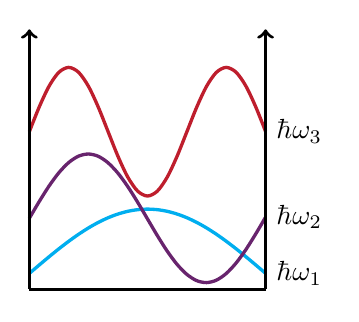
\begin{tikzpicture}
\begin{scope}[domain=0:3]
    \draw[draw=Blue, line width=1.2pt, smooth] plot (\x, { 0.2+ (2/3)^0.5 * sin(3.14 * \x r/ 3)}) node[right] {$\hbar \omega_1$}; 
    \draw[draw=Purple, line width=1.2pt,smooth] plot (\x, {0.9+ (2/3)^0.5 * sin(2* 3.15 * \x r/ 3)})  node[right]{$\hbar \omega_2$}; 
    \draw[draw=Red, line width=1.2pt, smooth] plot (\x, {2+ (2/3)^0.5 * sin(3* 3.14 * \x r / 3)}) node[right] {$\hbar \omega_3$}; 
    \draw[line width=1.2pt, ->] (0,0) -- (0,3.3);
    \draw[line width=1.2pt, ->] (3,0) -- (3,3.3);
    \draw[line width=1.2pt] (0,0) -- (3,0);
\end{scope}
\end{tikzpicture}
\caption{Infinite Quantum Well}
\end{figure}

\column{0.5\textwidth}
\begin{figure}
\centering
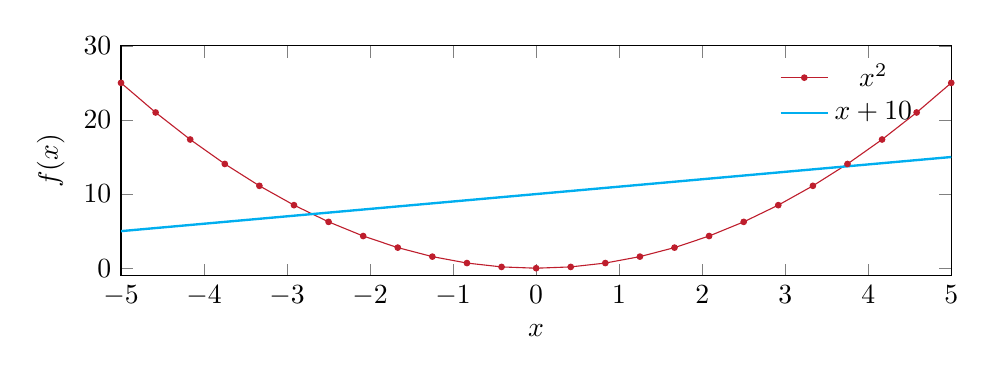
\begin{tikzpicture}
\begin{axis}[name=plot1,
    height=4.5cm,width=\linewidth,
    ylabel= {$f(x)$},
    xlabel= {$x$},
    ymin=-1.0, ymax=30,
    xmin=-5, xmax=5,
    legend style={draw=none,fill=none},
    legend pos=north east,
    ]
    \addplot[color=Red, mark=* ,mark options={scale=0.5,solid}] {x^2};
    \addlegendentry{$x^2$}
    \addplot[line width=0.3mm, Blue] {x + 10};
    \addlegendentry{$x+10$}
\end{axis}
\end{tikzpicture}
\caption{Some plots}
\end{figure}
\end{columns}
\end{frame}

%===============================================
\section{Second Main Section}

\subsection{Subsection}

\begin{frame}{Third Slide Title}{Blocks, Theorem and Examples}
\begin{block}{Block Title}
Block by definition produces a purple block with it's own title.
\end{block}
\begin{theorem}
Theorem by definition produces a red block with the title Theorem and italic text.
\end{theorem}
\begin{example}
Example by definition produces a blue block with the title Example.
\end{example}
\end{frame}

%===============================================
\section{Third Main Section}

\subsection{Subsection}

\begin{frame}{Fourth Slide Title}{Tables}
Here is a table!

\begin{center}
% Adjust size of the minipage if needed 
\begin{minipage}{0.5\textwidth}
\begin{block}{~\vspace{0.6cm}}
\begin{center}
\vspace{-0.6cm}
\begin{tabular}{c c c}
 \textcolor{white}{\textbf{Head 1}} & \textcolor{white}{\textbf{Head 2}} & \textcolor{white}{\textbf{Head 3}} \\~\\
  cell 1.1 & cell 1.2 & cell 1.3\\ 
  cell 2.1 & cell 2.2 & cell 2.3\\
  cell 3.1 & cell 3.2 & cell 3.3\\
  cell 4.1 & cell 4.2 & cell 4.3
\end{tabular}
\end{center}
\end{block}
\end{minipage}
\end{center}

\end{frame}

\begin{frame}{Fifth Slide Title}{Equations}

Here is the time-dependent Schr\"{o}dinger equation:

\begin{equation}
    i \hbar \frac{\partial }{\partial t} \Psi ( \mathbf{r}, t) = 
    \left[ - \frac{\hbar^2 }{2 m} \nabla^2 +V ( \mathbf{r}, t)  \right] \Psi ( \mathbf{r}, t).
\end{equation}

\end{frame}

%===============================================
\section{Final Comments}

% Use \alert{} to put the text in emphasis 
\begin{frame}{Summary}
  \begin{itemize}
  \item
    The \alert{first main message} of your presentation.
  \item
    The \alert{second main message} of your presentation.
  \end{itemize}
  
\vspace{1cm}

  \begin{itemize}
  \item
    Outlook
    \begin{itemize}
    \item
      To do in the future.
    \item
      Also to do in the future.
    \end{itemize}
  \end{itemize}
\end{frame}

%=====================================
% Further information, extra slides, etc

\begin{frame}{For Further Reading}
    
  \begin{thebibliography}{10}
    
  \beamertemplatebookbibitems
  % Book symbol

  \bibitem{Author1990}
    A.~Author.
    \newblock {\em Book title}.
    \newblock Editor, Year.
 
  \beamertemplatearticlebibitems
  % Article symbol

  \bibitem{Author1}
    A.~Author.
    \newblock Article title 1.
    \newblock {\em Journal A}, \textbf{number}, page (year).
    
 \bibitem{Author2}
    B.~Author.
    \newblock Article title 2.
    \newblock {\em Journal B}, \textbf{number}, page (year).
    
  \end{thebibliography}
\end{frame}

\end{document}
